\section{Data Analysis}
\subsection{Analyzing Window Size}

The findings on how window size influences classifier performance closely align with the original authors' observations on both the INRIA and Caltech datasets \cite{dalal_2005_histograms}. Larger window sizes capture more contextual information about the pedestrian and surrounding area, which explains why the largest window size of (128, 96) outperformed all other configurations on these datasets, as evident in figures \ref{fig:window_size_inria} and \ref{fig:window_size_caltech}.

In contrast, the PnPLO dataset exhibited a different trend, with the two smallest windows ((112, 48) and (100, 50)) achieving the highest performance scores. This is likely due to the fact that smaller windows are better able to focus on local features rather than global context, reducing the amount of potentially "confusing" information. It may also be the case that larger window sizes cause the classifier to overfit to the artificial characteristics of mannequins and statues (like display platforms) in the PnPLO dataset, leading to worse performance on this independent test set.


% Noting how this could inform practical applications - for example, a security system might want larger windows for detecting real pedestrians, while a museum inventory system cataloging statues might benefit from smaller windows

\subsection{Analyzing Derivative Masks}

The holistic derivative mask (HDM) proposed in Section \ref{sec:deriv_mask} significantly enhanced performance on both the Caltech (Figure \ref{fig:hdm_caltech}) and PnPLO (Figure \ref{fig:hdm_pnplo}) datasets. Nearly every configuration using HDM outperformed its counterpart without HDM (Figure \ref{fig:hdm_total}). The HDM approach preserves gradient information at object boundaries, which is crucial for detecting pedestrians in low-resolution images like those in the Caltech dataset \cite{dollar_2009_pedestrian}.

The performance difference on the INRIA dataset (Figure \ref{fig:hdm_inria}) is less pronounced, which is unsurprising given that pedestrians in INRIA are typically centered with ample surrounding margin \cite{dalal_2005_histograms}. Even so, the best-performing INRIA configuration with HDM still outperforms the best configuration without HDM with statistical significance ($p=6\cdot 10^{-9}$), as shown in Figure \ref{fig:best_hdm_inria}

\begin{figure}
    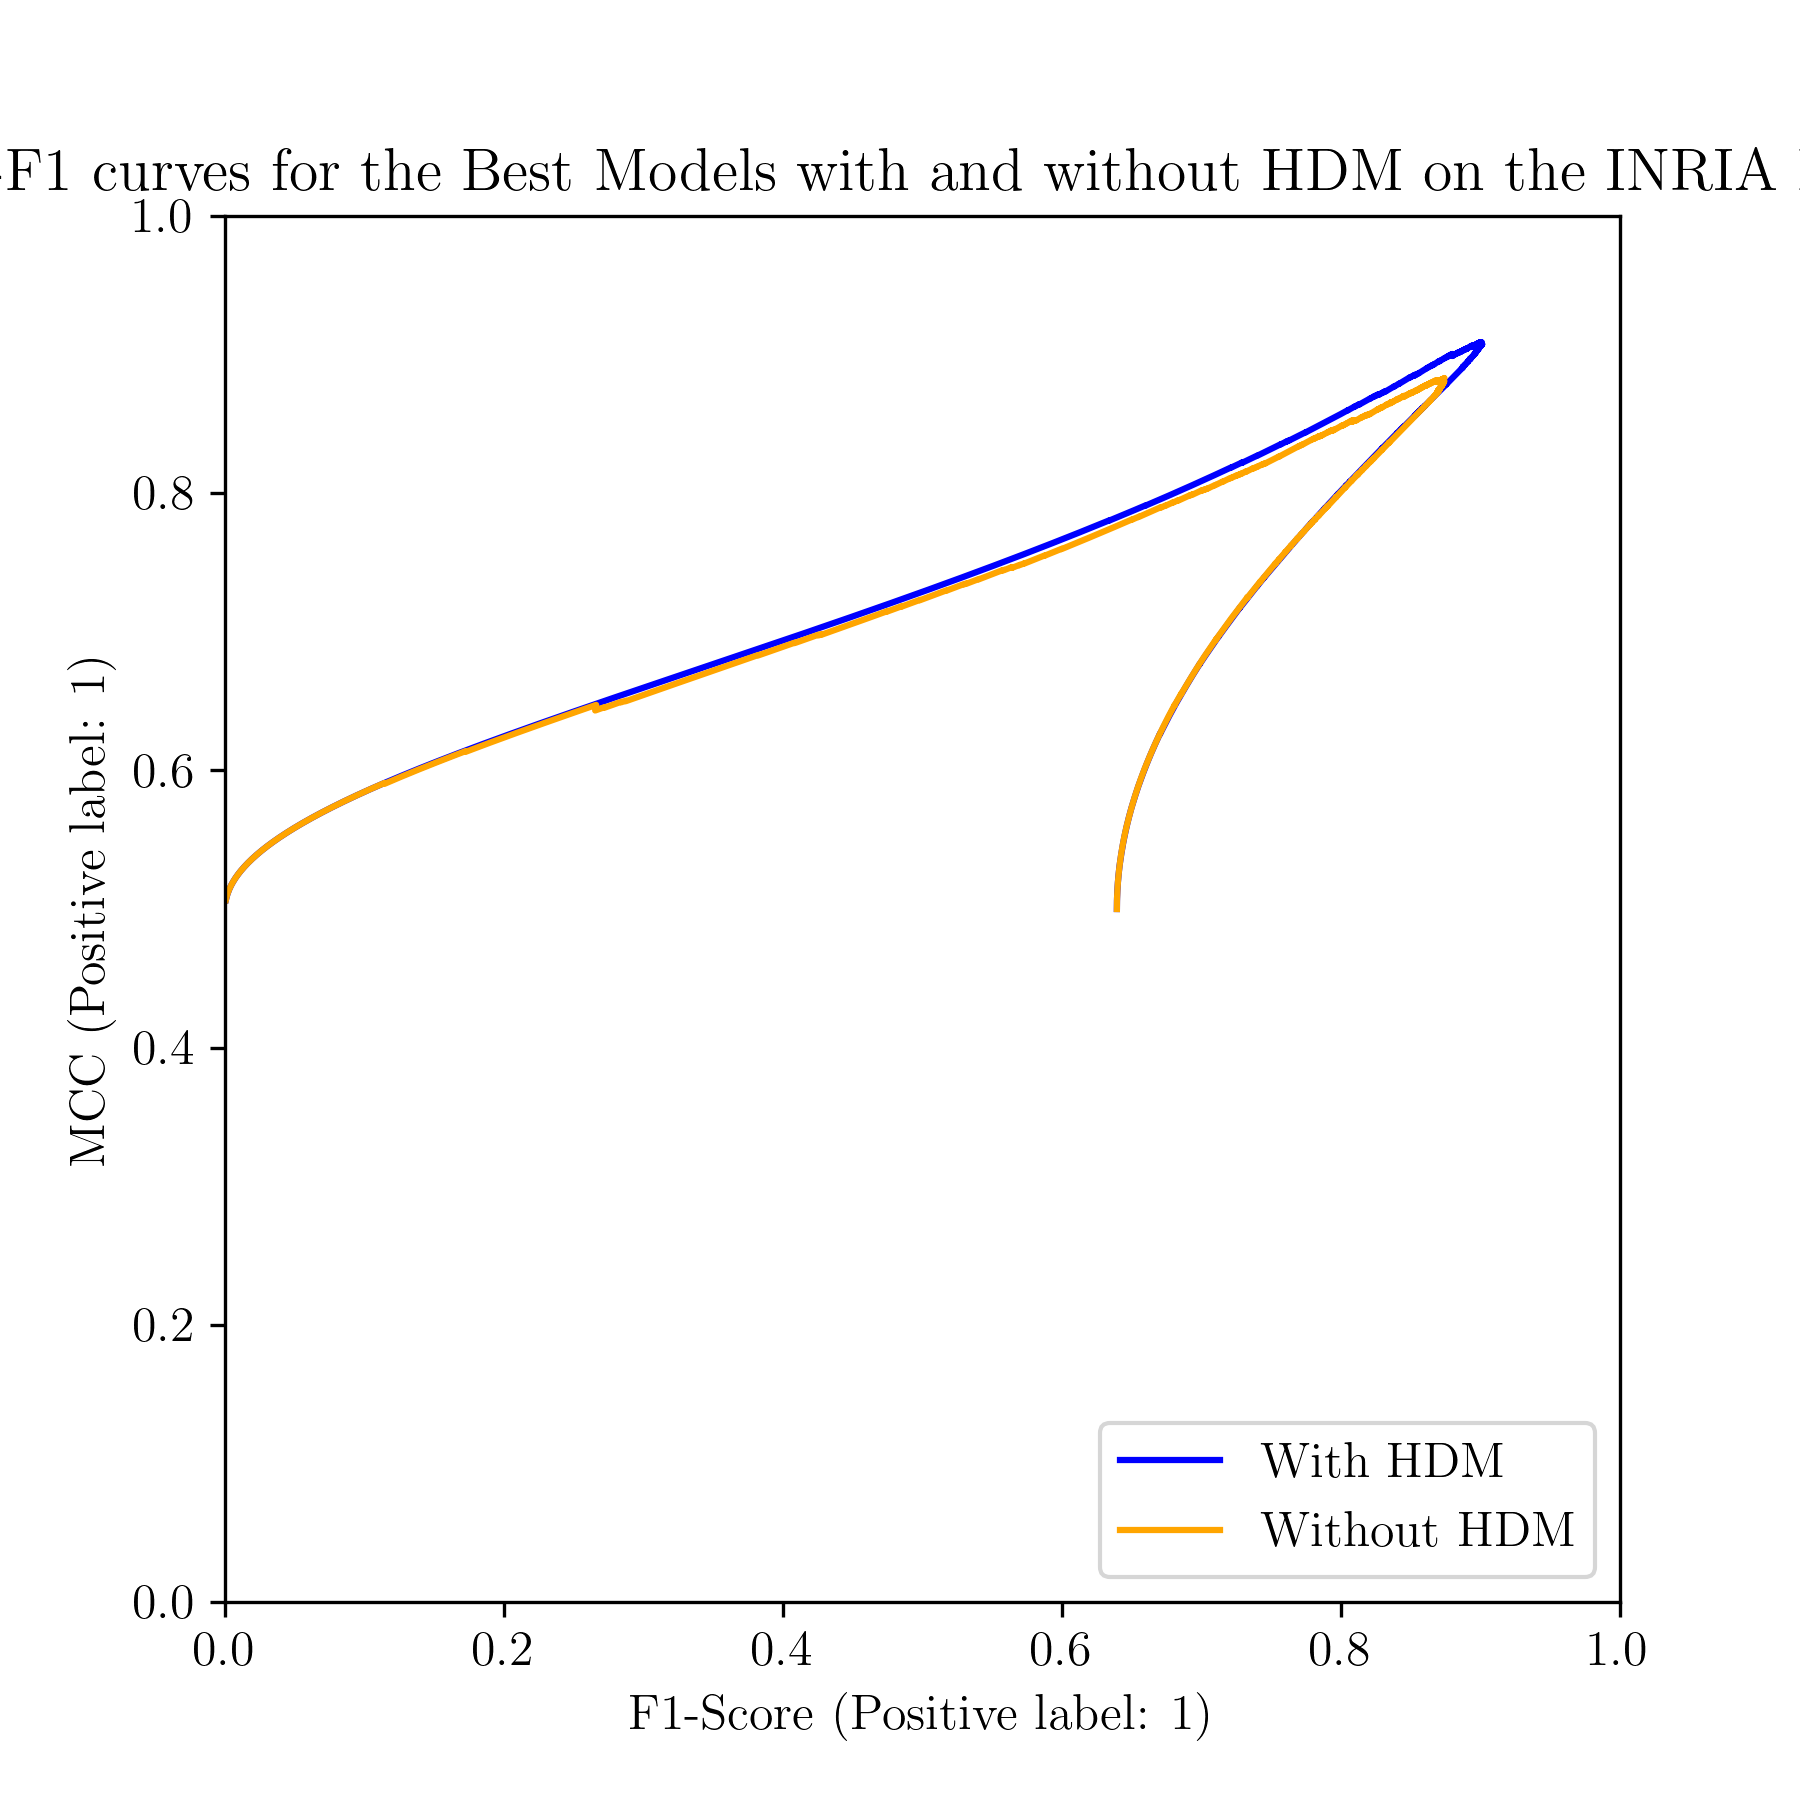
\includegraphics[width=0.6\linewidth]{best_hdm_mcc_f1_inria.png}
    \caption{
        The best performing configurations on the INRIA data set with and without the holistic derivative mask (HDM). 
    }
    \label{fig:best_hdm_inria}
\end{figure}


\subsection{Analyzing Orientation Bin Sizes}

The experimental results shown in figures \ref{fig:orientation_bins_inria} through \ref{fig:orientation_bins_total} align with Dalal and Triggs' seminal HOG paper \cite{dalal_2005_histograms}: increasing the number of orientation bins beyond 9 yields minimal performance improvements (all pairwise p-values $\sim 0.05$). This demonstrates the law of diminishing returns in pedestrian detection, which can be attributed to the relatively consistent edge orientations in human body shapes. Finer orientation binning over the 0°-180° range (such as 13.8° intervals for 13 bins or 10° intervals for 18 bins) fails to capture significantly more discriminative information. While increasing bin count raises feature vector dimensionality (discussed in section \ref{sec:feature_vector_dimensionality}), which could theoretically degrade performance, our experiments show no such negative impact. In fact, configurations with 18 bins show marginally better performance than those with fewer bins, though this improvement is less influential than parameters such as window size or derivative mask selection.

\subsection{Analyzing Block Density}

The results derived from the heatmaps in figures \ref{fig:cell_block_heatmap_inria} through \ref{fig:cell_block_heatmap_total} diverge from those reported by Dalal and Triggs \cite{dalal_2005_histograms}. Our analysis reveals that the optimal block density configuration for both INRIA and PnPLO datasets consistently comprises a (2,2) block size and (8,8) cell size. The Caltech dataset exhibits a similar trend, though interestingly, the density configuration of (4,4) block size and (4,4) cell size performs in an identical manner ($p=0.775$). Both these configurations yield a block area of 16$\times$16 pixels, which appears to provide the optimal balance between capturing local spatial information and maintaining global context, as illustrated in figure \ref{fig:block_area}. This finding suggests that a 16$\times$16 pixel block area offers the best trade-off for pedestrian detection across diverse datasets. Notably, larger block sizes tend to lose focus on the critical local features that define a pedestrian, while smaller block sizes, like (1,1), fail to capture the broader contextual information necessary for distinguishing pedestrians from their surroundings. 

\begin{figure}
    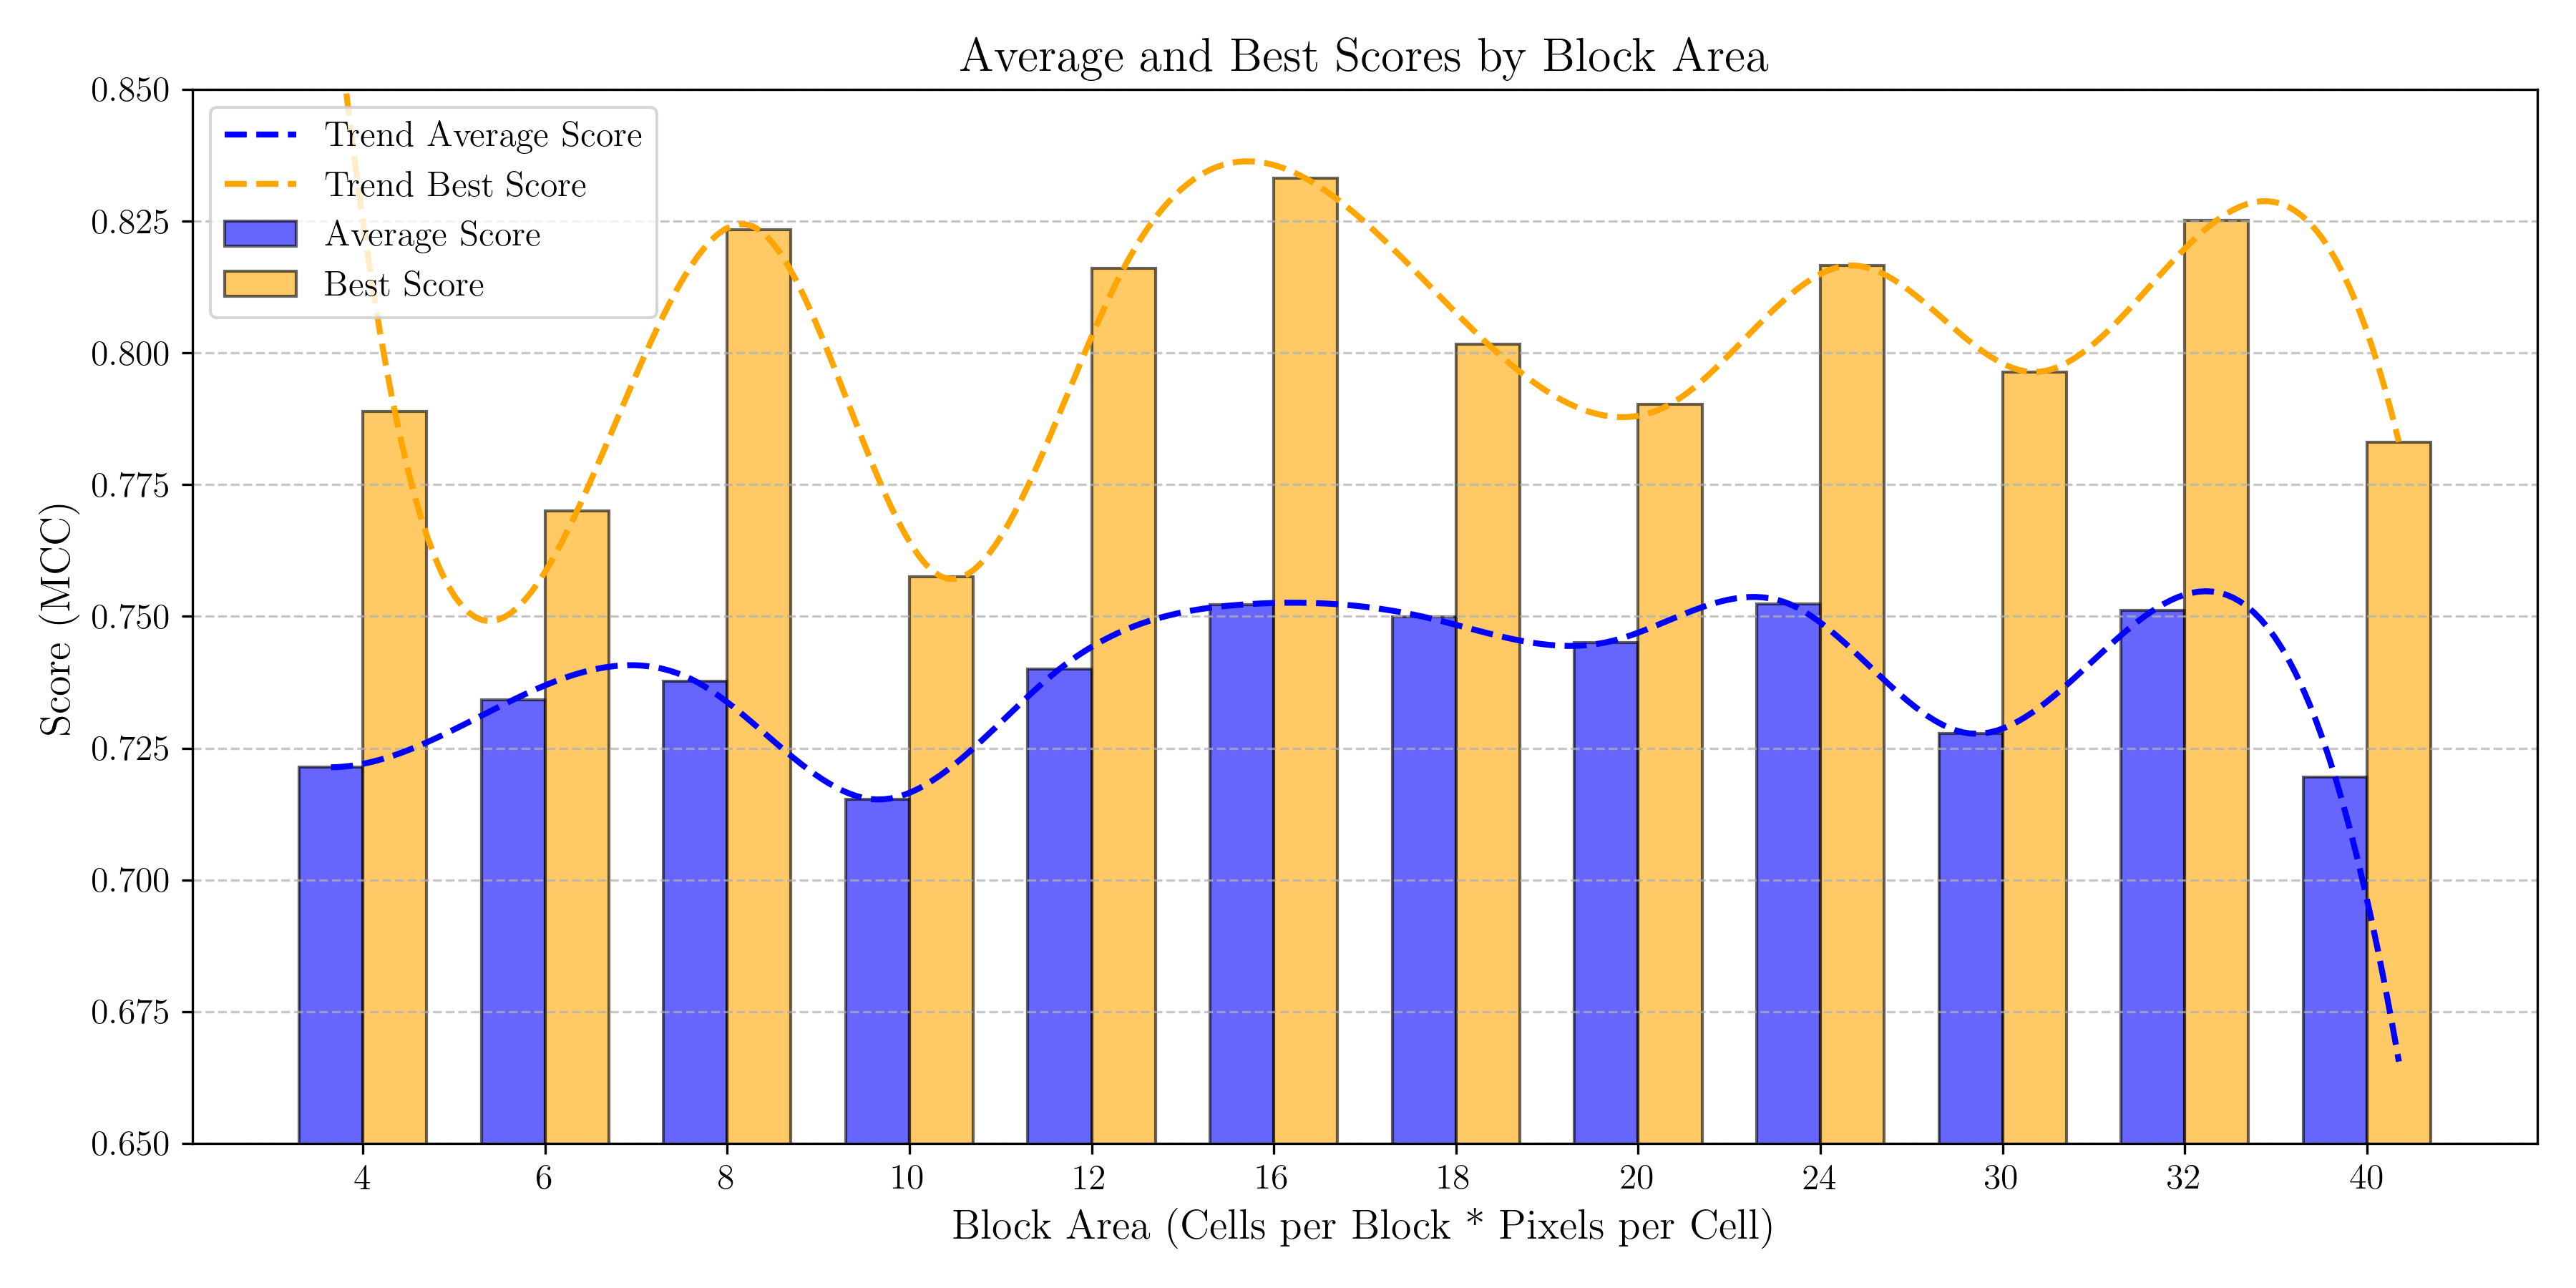
\includegraphics[width=\linewidth]{mcc_block_area.png}
    \caption{
        A bar chart of average and best MCC scores for each configuration's block area (defined as block width (or height) $\times$ cell width (or height)). 
    }
    \label{fig:block_area}
\end{figure}

Interestingly, the (10,10) cell size configuration consistently underperforms across all datasets, aligning with established HOG principles for pedestrian detection \cite{dalal_2005_histograms}. Our findings indicate that cell sizes beyond (8,8) provide overly coarse resolutions, failing to capture the fine-grained spatial information crucial for distinguishing pedestrians from their surroundings. The (8,8) cell size emerges as optimal, striking a delicate balance between detail preservation and computational efficiency. This balance is particularly significant as an increase in cell size leads to a decrease in feature vector dimensionality, as shown in equation \ref{vector_dimensions}, which directly correlates with reduced computation time, as illustrated in figure \ref{fig:correlation_with_best_fit}. 

\begin{figure}
    \includesvg[width=\linewidth]{correlation_with_best_fit.svg}
    \caption{
        A scatter plot of the correlation between dimensionality and time of computation, with a best-fit line.
    }
    \label{fig:correlation_with_best_fit}
\end{figure}


\subsection{Analyzing Block Stride}

The findings regarding block stride values closely align with those reported by the original HOG authors \cite{dalal_2005_histograms}. Figures \ref{fig:overlap_2_2} through \ref{fig:overlap_4_4} almost consistently show that higher stride values, which result in greater block overlap, significantly improve detection performance. Specifically, for (4, 4) blocks, our experiments reveal a statistically significant performance improvement ($p=0.000534$) when using 75\% overlap (stride of 2) compared to 50\% overlap (stride of 4). This underscores the importance of block overlap in capturing local contrast normalization effectively. While a similarly significant increase in performance is observed for (3,3) blocks, (2,2) blocks exhibit no statistically significant difference between 50\% and 0\% overlap ($p=0.2911$), suggesting that it might be more optimal to use stride values (2,2) for (2,2) blocks as to decrease computational complexity without sacrificing detection accuracy.